\documentclass{beamer}

% Theme settings
\usetheme{Madrid}
\usecolortheme{default}
\setbeamertemplate{navigation symbols}{}
\setbeamertemplate{caption}[numbered]

% Packages
\usepackage{amsmath}
\usepackage{amsthm}
\usepackage{amsfonts}
\usepackage{amssymb}
\usepackage{graphicx}
\usepackage{hyperref}
\usepackage{booktabs}

% Title information
\title{Reservoir Computing: Implementation and Analysis}
\subtitle{Study Oriented Project}
\author{Vimarsh Shah}
\institute{Department of Physics \\ BITS Pilani, Goa}
\date{April 2025}

\begin{document}

% Title slide
\begin{frame}
\titlepage
\end{frame}

% Table of contents
\begin{frame}{Outline}
\tableofcontents
\end{frame}

% Introduction section
\section{Introduction}

\begin{frame}{Introduction to Reservoir Computing}
\begin{itemize}
\item Machine learning transforms fields by extracting patterns from data
\item Traditional deep learning often uses gradient-based optimization
\item Recurrent Neural Networks (RNNs) face challenges:
    \begin{itemize}
    \item Vanishing/exploding gradients
    \item Time-consuming training processes
    \end{itemize}
\item Reservoir Computing emerges as an efficient solution:
    \begin{itemize}
    \item Fixed, randomly initialized recurrent network (reservoir)
    \item Only output connections are trained
    \item Maintains representational power with simplified training
    \end{itemize}
\end{itemize}
\end{frame}

\begin{frame}{Key Advantages of Reservoir Computing}
\begin{itemize}
\item Simplified training through linear regression of output weights only
\item Reduced computational demands compared to full RNN training
\item Ability to process temporal information through the reservoir's inherent memory
\item Adaptability to physical implementations in various substrates
\end{itemize}
\end{frame}

\begin{frame}{Comparison with Other Neural Networks}
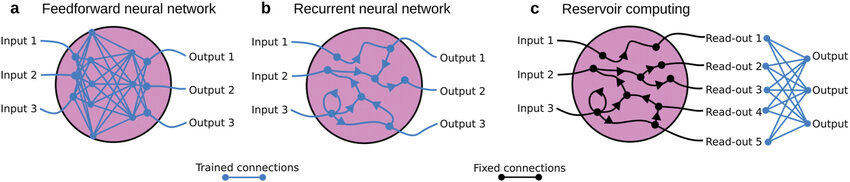
\includegraphics[width=1.0\linewidth]{figures/rc_difference_with others.png}
\caption{Illustration of (a) a feedforward neural network, (b) a recurrent neural network, and (c) a reservoir computing system}
\end{frame}

% Basics section
\section{Basics of Reservoir Computing}

\begin{frame}{General Principle}
\begin{itemize}
\item Transforms input signals through a high-dimensional, nonlinear dynamical system
\item Three main components:
    \begin{itemize}
    \item \textbf{Input Layer:} Maps external inputs to the reservoir 
    \item \textbf{Reservoir:} Random, fixed recurrent network
    \item \textbf{Output Layer:} Linear readout mechanism (trained)
    \end{itemize}
\item Input triggers complex dynamics within the reservoir
\item Temporal information preserved through recurrent connections
\end{itemize}
\end{frame}

\begin{frame}{Mathematical Formulation}
A typical discrete-time reservoir update:
\[
\mathbf{x}[n+1] = f\bigl(\mathbf{W}\mathbf{x}[n] + \mathbf{W}^{\mathrm{in}}\mathbf{u}[n] + \mathbf{b}\bigr)
\]

Where:
\begin{itemize}
\item $\mathbf{x}[n]\in \mathbb{R}^N$ is the reservoir state at time step $n$
\item $\mathbf{u}[n]$ is the input vector
\item $\mathbf{W}$ is the fixed, random reservoir weight matrix
\item $\mathbf{W}^{\mathrm{in}}$ couples the input
\item $f(\cdot)$ is a nonlinear activation function (e.g., $\tanh$)
\item $\mathbf{b}$ is a bias term
\end{itemize}

The output is formed as:
\[
\mathbf{y}[n] = \mathbf{W}^{\mathrm{out}}\bigl[\mathbf{x}[n];\,\mathbf{u}[n]\bigr]
\]

Only $\mathbf{W}^{\mathrm{out}}$ is adjusted during training.
\end{frame}

\begin{frame}{Echo State Property and Fading Memory}
\begin{itemize}
\item \textbf{Echo State Property (ESP)}: Ensures the reservoir's state depends only on history of inputs, not initial conditions
    \begin{itemize}
    \item Any influence of initial reservoir state eventually fades away
    \item System responds consistently to the same input sequence
    \end{itemize}
\item \textbf{Fading Memory}: Reservoir retains information about recent inputs
    \begin{itemize}
    \item Influence diminishes for inputs further in the past
    \item Essential for processing temporal information effectively
    \end{itemize}
\item Typically achieved by scaling the spectral radius of $\mathbf{W}$ to be less than unity
\end{itemize}
\end{frame}

\begin{frame}{Comparison with Traditional RNNs}
\begin{columns}
\begin{column}{0.5\textwidth}
\textbf{Traditional RNNs:}
\begin{itemize}
\item All connections trained (input, recurrent, output)
\item Uses backpropagation through time
\item Computationally intensive
\item May suffer from convergence issues
\end{itemize}
\end{column}
\begin{column}{0.5\textwidth}
\textbf{Reservoir Computing:}
\begin{itemize}
\item Only output connections trained
\item Typically uses simple linear regression
\item Input and recurrent connections remain fixed
\item Computationally efficient
\item Avoids vanishing/exploding gradients
\end{itemize}
\end{column}
\end{columns}
\end{frame}

\begin{frame}{Variants: Echo State Networks (ESNs)}
\begin{columns}
\begin{column}{0.5\textwidth}
\begin{itemize}
\item Introduced by Jaeger
\item Use rate-based neurons
\item Continuous activation functions (e.g., tanh)
\item Sparse random connectivity between reservoir units
\end{itemize}
\end{column}
\begin{column}{0.5\textwidth}
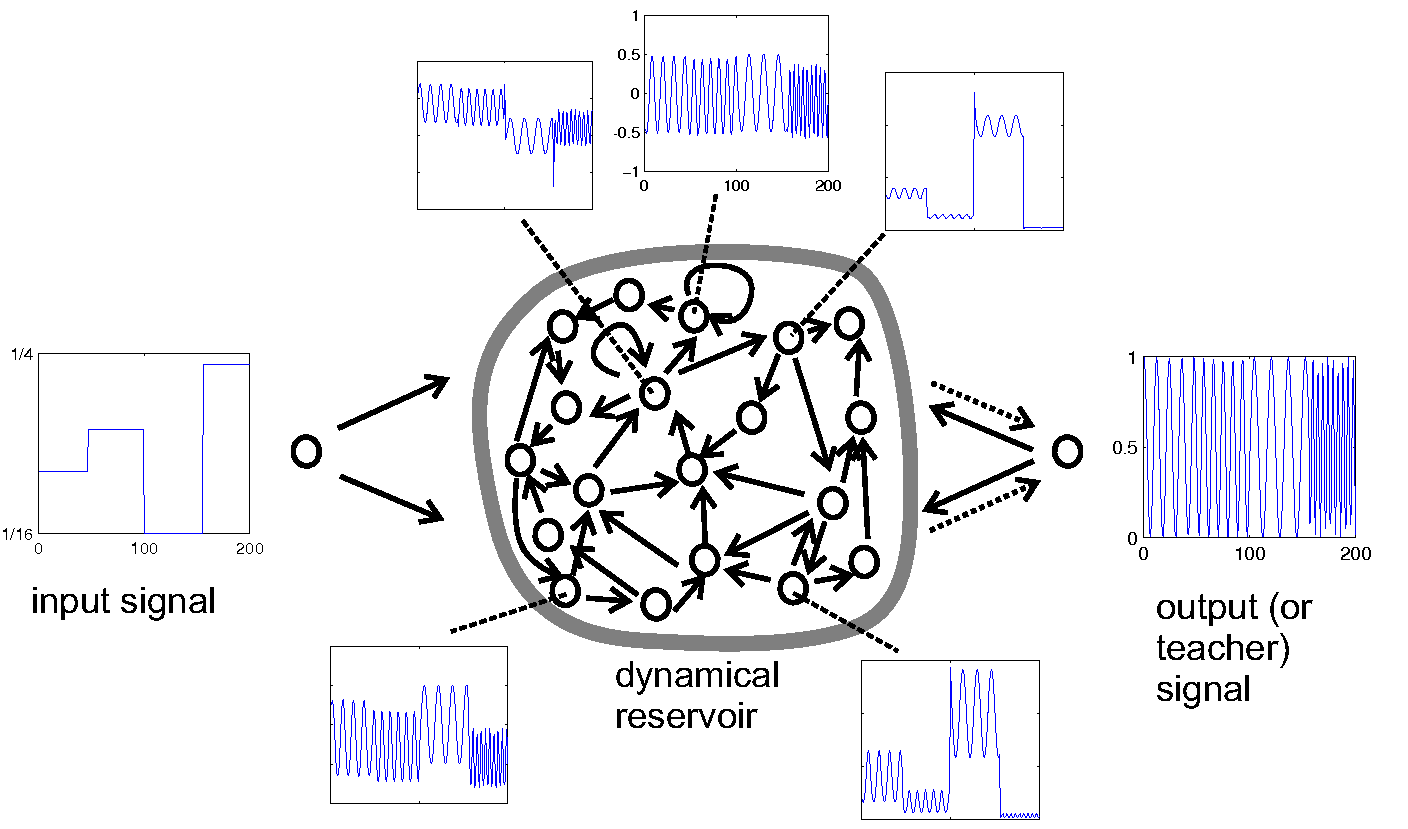
\includegraphics[width=1\linewidth]{figures/ESN_diag_FreqGenSchema.png}
\caption{Echo State Network diagram}
\end{column}
\end{columns}
\end{frame}

\begin{frame}{Variants: Liquid State Machines (LSMs)}
\begin{columns}
\begin{column}{0.5\textwidth}
\begin{itemize}
\item Developed by Maass et al.
\item Use spiking neuron models
\item More closely resemble biological neurons
\item Initially conceived in computational neuroscience
\end{itemize}
\end{column}
\begin{column}{0.5\textwidth}
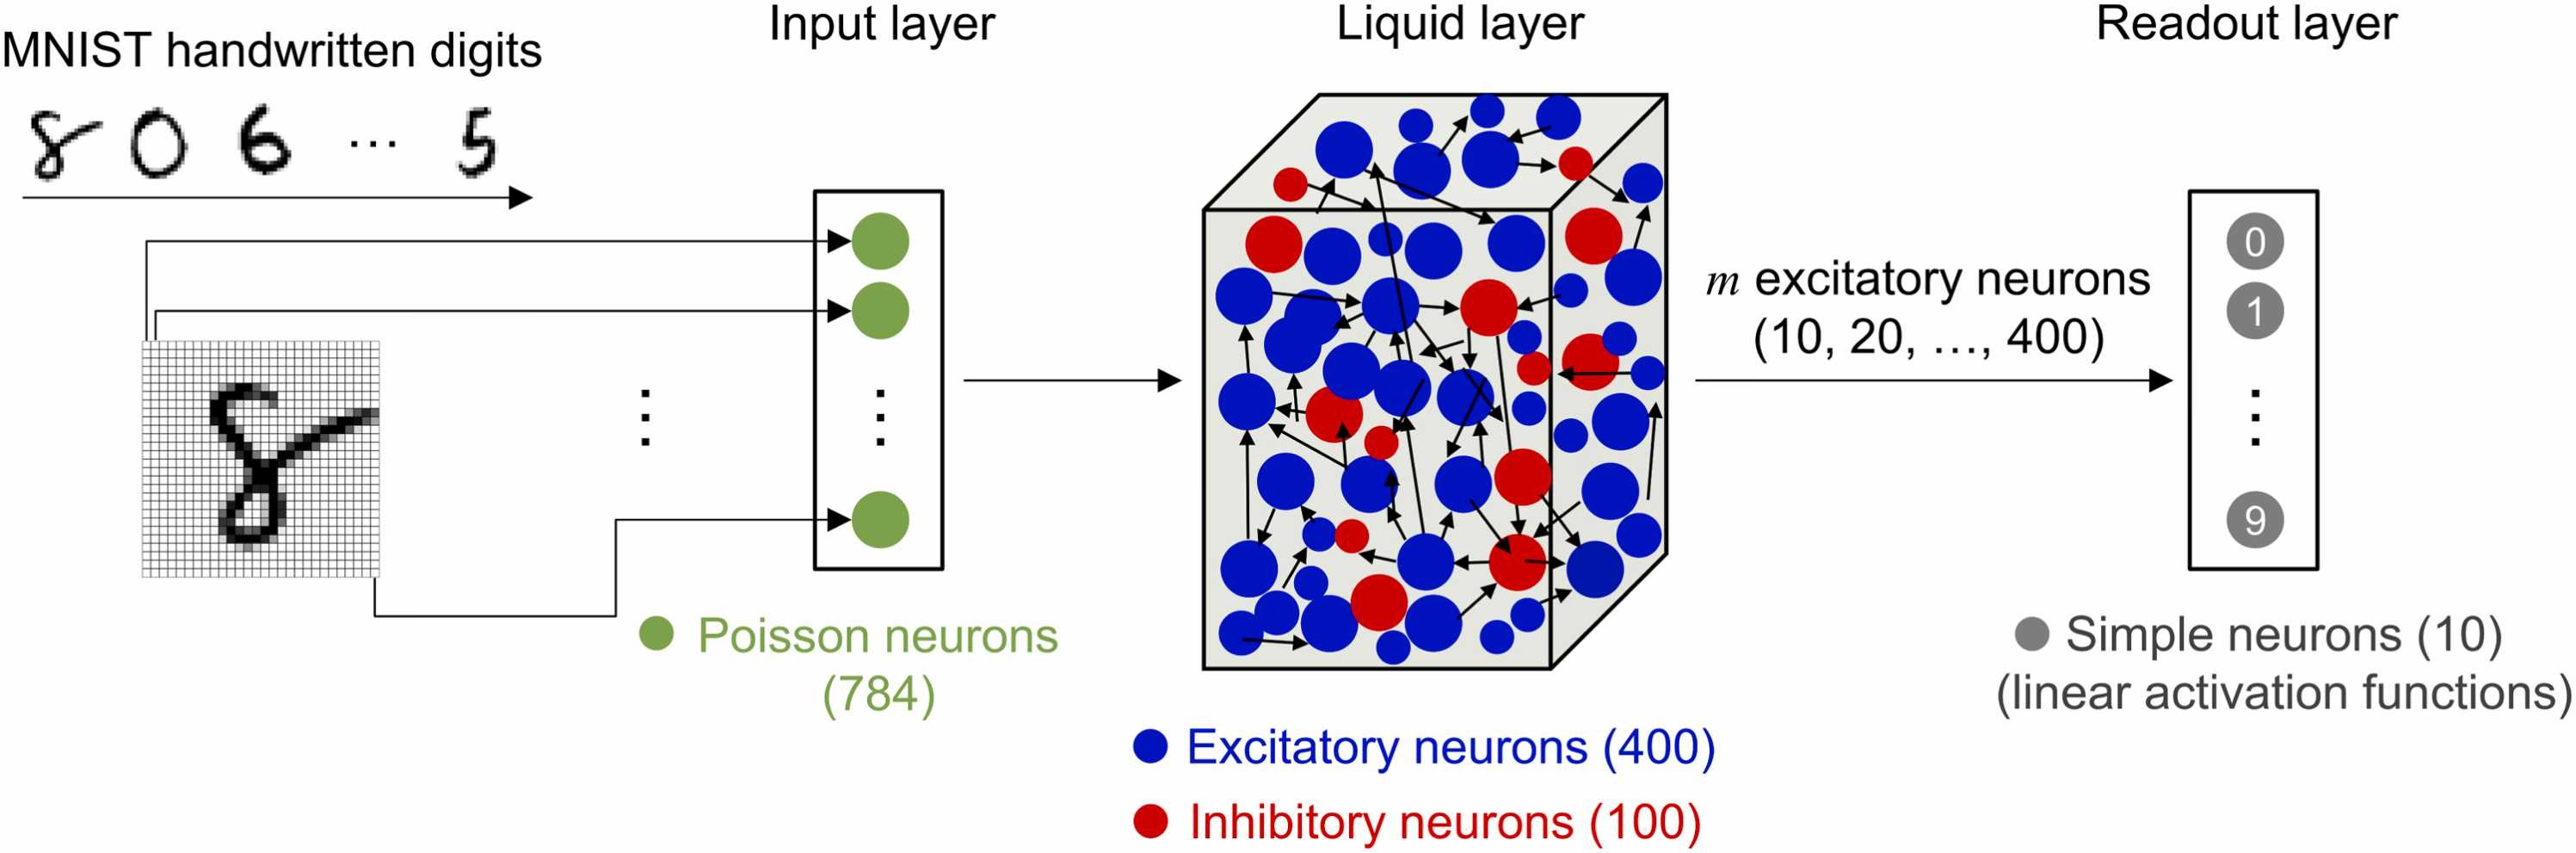
\includegraphics[width=1\linewidth]{figures/lsm_diag.png}
\caption{Liquid State Machine diagram}
\end{column}
\end{columns}
\end{frame}

\begin{frame}{Training Methodology}
\begin{itemize}
\item Much simpler than traditional neural networks:
    \begin{enumerate}
    \item Feed input signals into the reservoir 
    \item Collect resulting reservoir states
    \item Train linear readout function (ridge regression)
    \item Apply trained readout to new reservoir states
    \end{enumerate}
\item Mathematical formulation:
\[
W_{\text{out}} = YG^T\left(GG^T + \lambda I\right)^{-1}
\]
\item Where $W_{out}$ = output weights, $Y$ = target outputs, $G$ = reservoir states, $\lambda$ = regularization parameter, $I$ = identity matrix
\end{itemize}
\end{frame}

\begin{frame}{Advantages and Limitations}
\begin{columns}
\begin{column}{0.5\textwidth}
\textbf{Advantages:}
\begin{itemize}
\item Training involves only linear regression
\item Same reservoir usable for multiple tasks
\item Fixed reservoir enables physical implementation
\end{itemize}
\end{column}
\begin{column}{0.5\textwidth}
\textbf{Limitations:}
\begin{itemize}
\item Limited control due to random initialization
\item Memory capacity constrained by reservoir size
\item Performance varies based on task-reservoir match
\item Highly dependent on hyperparameters
\end{itemize}
\end{column}
\end{columns}
\end{frame}

% Literature Review section
\section{Literature Review}

\begin{frame}{Literature Review}
\begin{itemize}
\item \textbf{Brunner et al. (2022)}: Explored RC fundamentals and setup methodology
\item \textbf{Carroll \& Pecora (2022)}: Identified "Catch-22s" in standard RC models
    \begin{itemize}
    \item Basin prediction in multistable systems requires long warm-up
    \item NGRC variant performs better but requires precise system knowledge
    \end{itemize}
\item \textbf{Arun et al. (2024)}: Used discrete nonlinear map as reservoir
    \begin{itemize}
    \item Logistic map with trigonometric series for virtual nodes
    \item Effective for predicting various benchmark systems
    \end{itemize}
\end{itemize}
\end{frame}

\begin{frame}{Literature Review (continued)}
\begin{itemize}
\item \textbf{Mandal et al. (2022)}: Physical example of minimal reservoir
    \begin{itemize}
    \item Single driven pendulum as reservoir
    \item Exploited pendulum's rich transient dynamics
    \item Even one-dimensional system achieved good accuracy
    \end{itemize}
\item \textbf{Itoh et al. (2020)}: Reconstructing bifurcation diagrams from data
    \begin{itemize}
    \item Generated time-series from electronic circuit
    \item Used Extreme Learning Machine (ELM) to train predictor
    \item Successfully reconstructed system's bifurcation diagram
    \item Method proved robust even with noisy conditions
    \end{itemize}
\end{itemize}
\end{frame}

% Implementation and Results section
\section{Implementation and Results}

\begin{frame}{Pendulum Reservoir}
The driven damped pendulum dynamics:
\begin{equation}
\begin{aligned}
\frac{dx}{dt} &= v, \\
\frac{dv}{dt} &= -\frac{g}{l} \sin(x) - k v + f \, \text{sign}(\sin(\omega t))
\end{aligned}
\end{equation}

Where:
\begin{itemize}
\item $x(t)$ = angular displacement
\item $v(t)$ = angular velocity
\item $g$ = gravitational acceleration
\item $l$ = pendulum length
\item $k$ = damping coefficient
\item $f$ = external forcing amplitude
\item $\omega$ = forcing frequency
\end{itemize}
\end{frame}

\begin{frame}{Pendulum Reservoir Results}
\begin{figure}
\centering
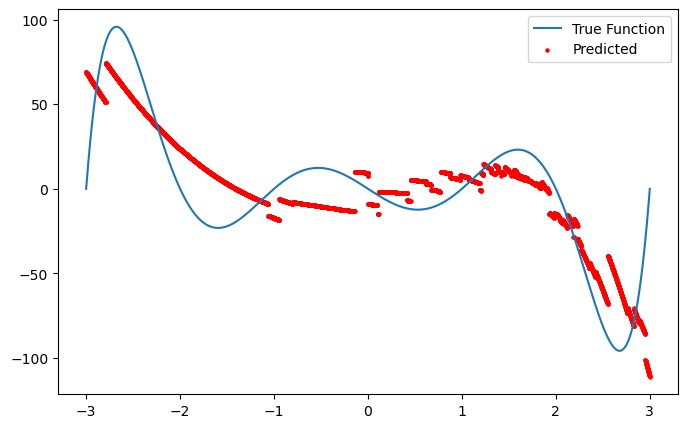
\includegraphics[width=0.75\linewidth]{figures/pendulum_result_0.png}
\caption{Results of the single pendulum reservoir experiment}
\end{figure}
\end{frame}

\begin{frame}{Pendulum Reservoir: Lorenz System}
Lorenz system equations:
\begin{equation}
\begin{aligned}
\frac{dx}{dt} &= \sigma (y - x), \\
\frac{dy}{dt} &= x (\rho - z) - y, \\
\frac{dz}{dt} &= x y - \beta z
\end{aligned}
\end{equation}

With standard parameters: $\sigma = 10$, $\rho = 28$, $\beta = \frac{8}{3}$
\end{frame}

\begin{frame}{Pendulum Reservoir: Lorenz System Results}
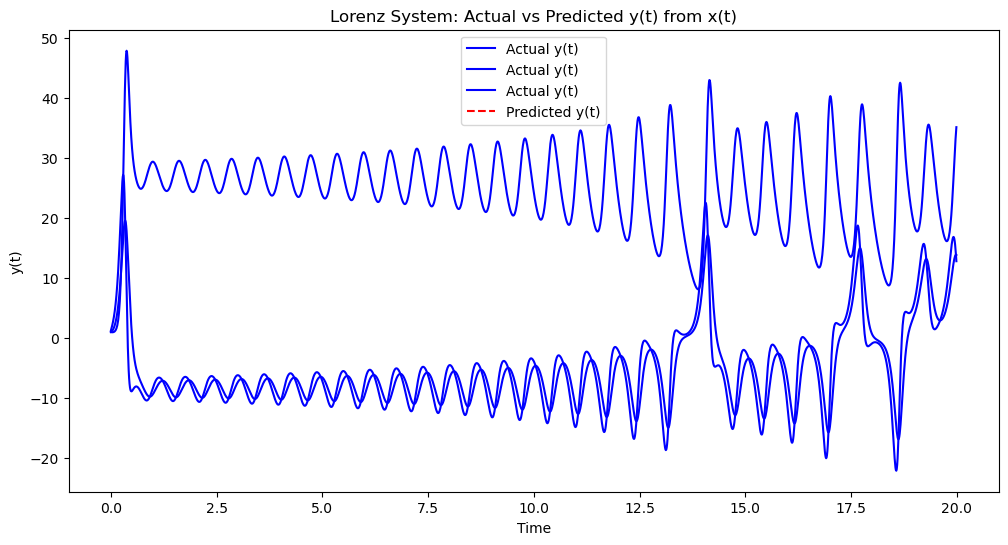
\includegraphics[width=1\linewidth]{figures/lorentz_pendulum_1.png}
\caption{Actual vs Predicted for the Lorenz system using Pendulum reservoir}
\end{frame}

\begin{frame}{Pendulum Reservoir: 3D Visualization}
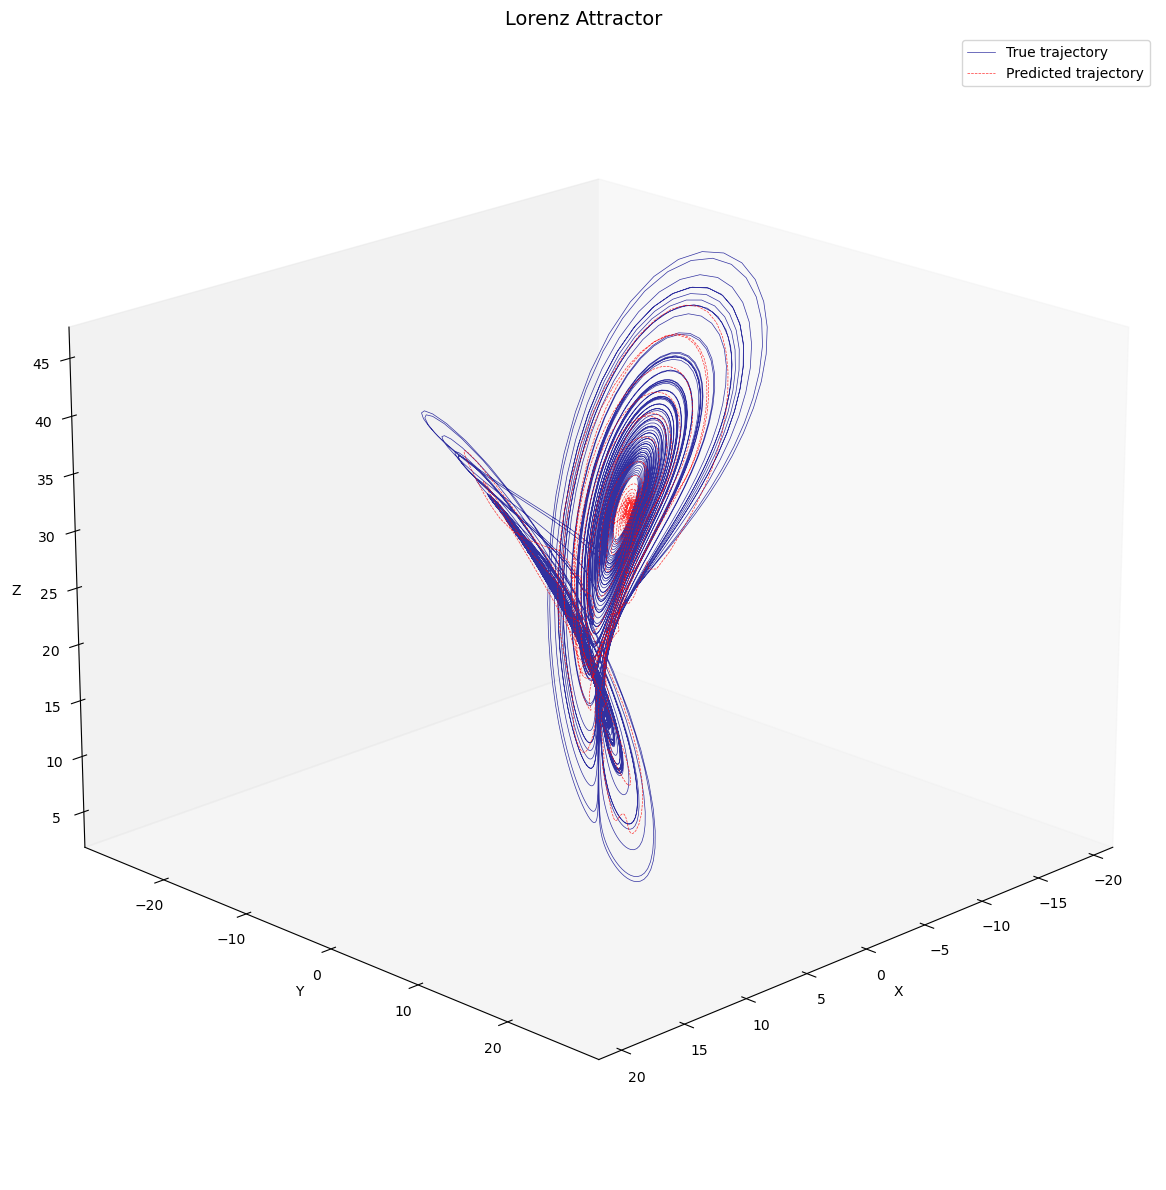
\includegraphics[width=1\linewidth]{figures/lorentz_pendulum_2.png}
\caption{3D render of actual vs Predicted timestep}
\end{frame}

\begin{frame}{Logistic Map Reservoir}
\begin{itemize}
\item Constructed following Arun et al. (2024)
\item Logistic map: $x_{n+1} = r x_n (1-x_n)$
\item Used \emph{virtual nodes} technique:
    \begin{itemize}
    \item Iterate map several times per input
    \item Sample intermediate values
    \item Combine with trigonometric expansion
    \end{itemize}
\item Tested on 7th-degree polynomial benchmark
\end{itemize}
\end{frame}

\begin{frame}{Logistic Map Reservoir Results}
\begin{figure}
\centering
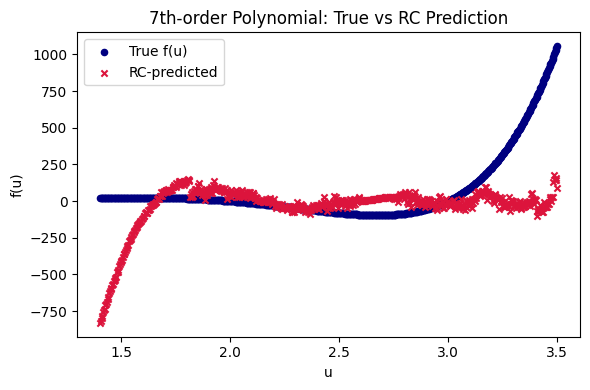
\includegraphics[width=0.75\linewidth]{figures/logistic_7th_degree.png}
\caption{Results using Logistic Map to map to a target polynomial}
\end{figure}
\end{frame}

\begin{frame}{Logistic Map: Lorenz System Results}
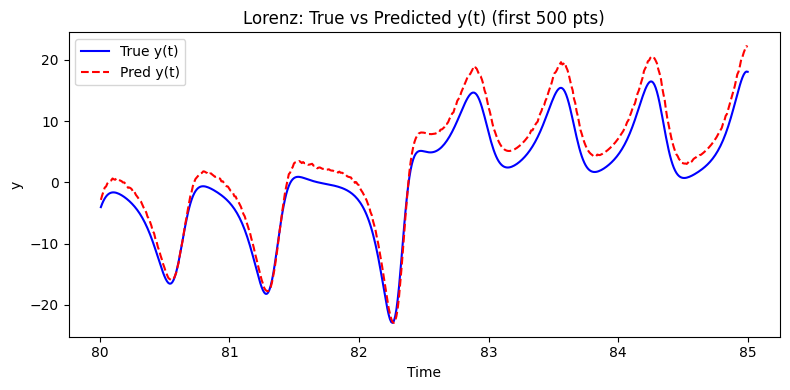
\includegraphics[width=1\linewidth]{figures/lorentz_logistic_pred_true.png}
\caption{Results for the Lorenz attractor using Logistic Map}
\end{frame}

\begin{frame}{Logistic Map: Evolution over Time}
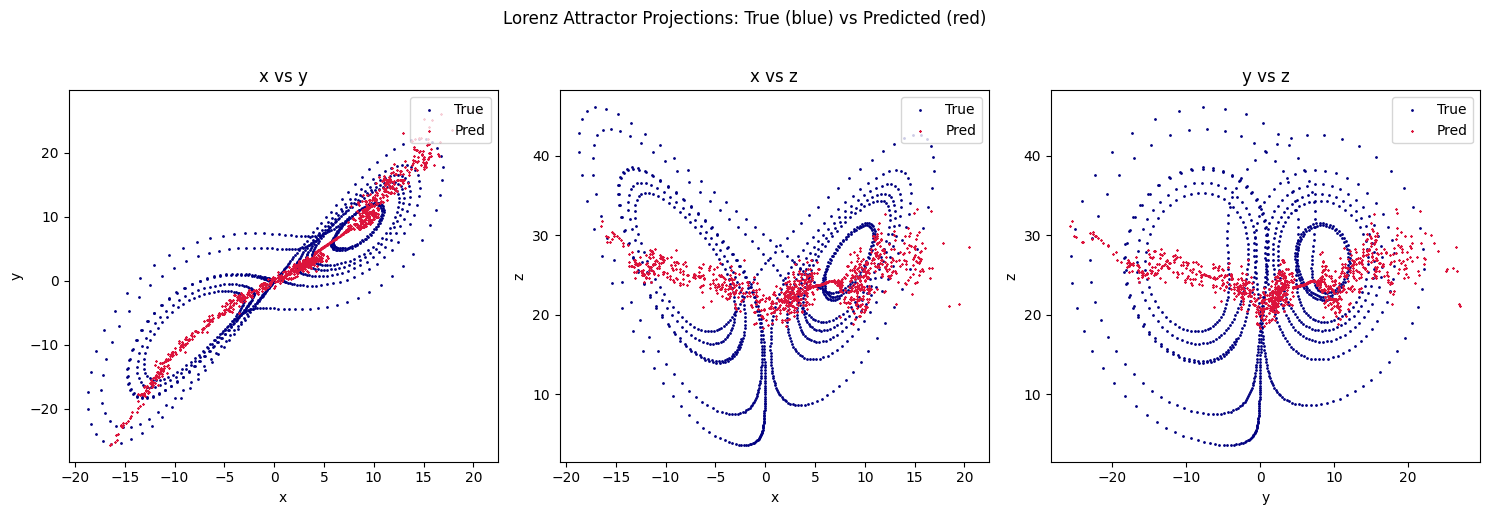
\includegraphics[width=1\linewidth]{figures/lorenz_logistic_pred_diagram.png}
\caption{Results for the Lorenz attractor using Logistic Map, evolution of different axes over time}
\end{frame}

\begin{frame}{Bifurcation Reconstruction via PCA and ELM}
\begin{itemize}
\item Inspired by Itoh et al. (2020)
\item Procedure:
    \begin{itemize}
    \item Run simulations across parameter range $\mu$
    \item Feed time-series data through reservoir
    \item Apply PCA to reduce dimensionality
    \item Train ELM regressor to map features to predicted output
    \item Sweep parameter $\mu$ and trace transitions
    \end{itemize}
\end{itemize}
\end{frame}

\begin{frame}{Bifurcation Reconstruction: Initial Results}
\begin{figure}
\centering
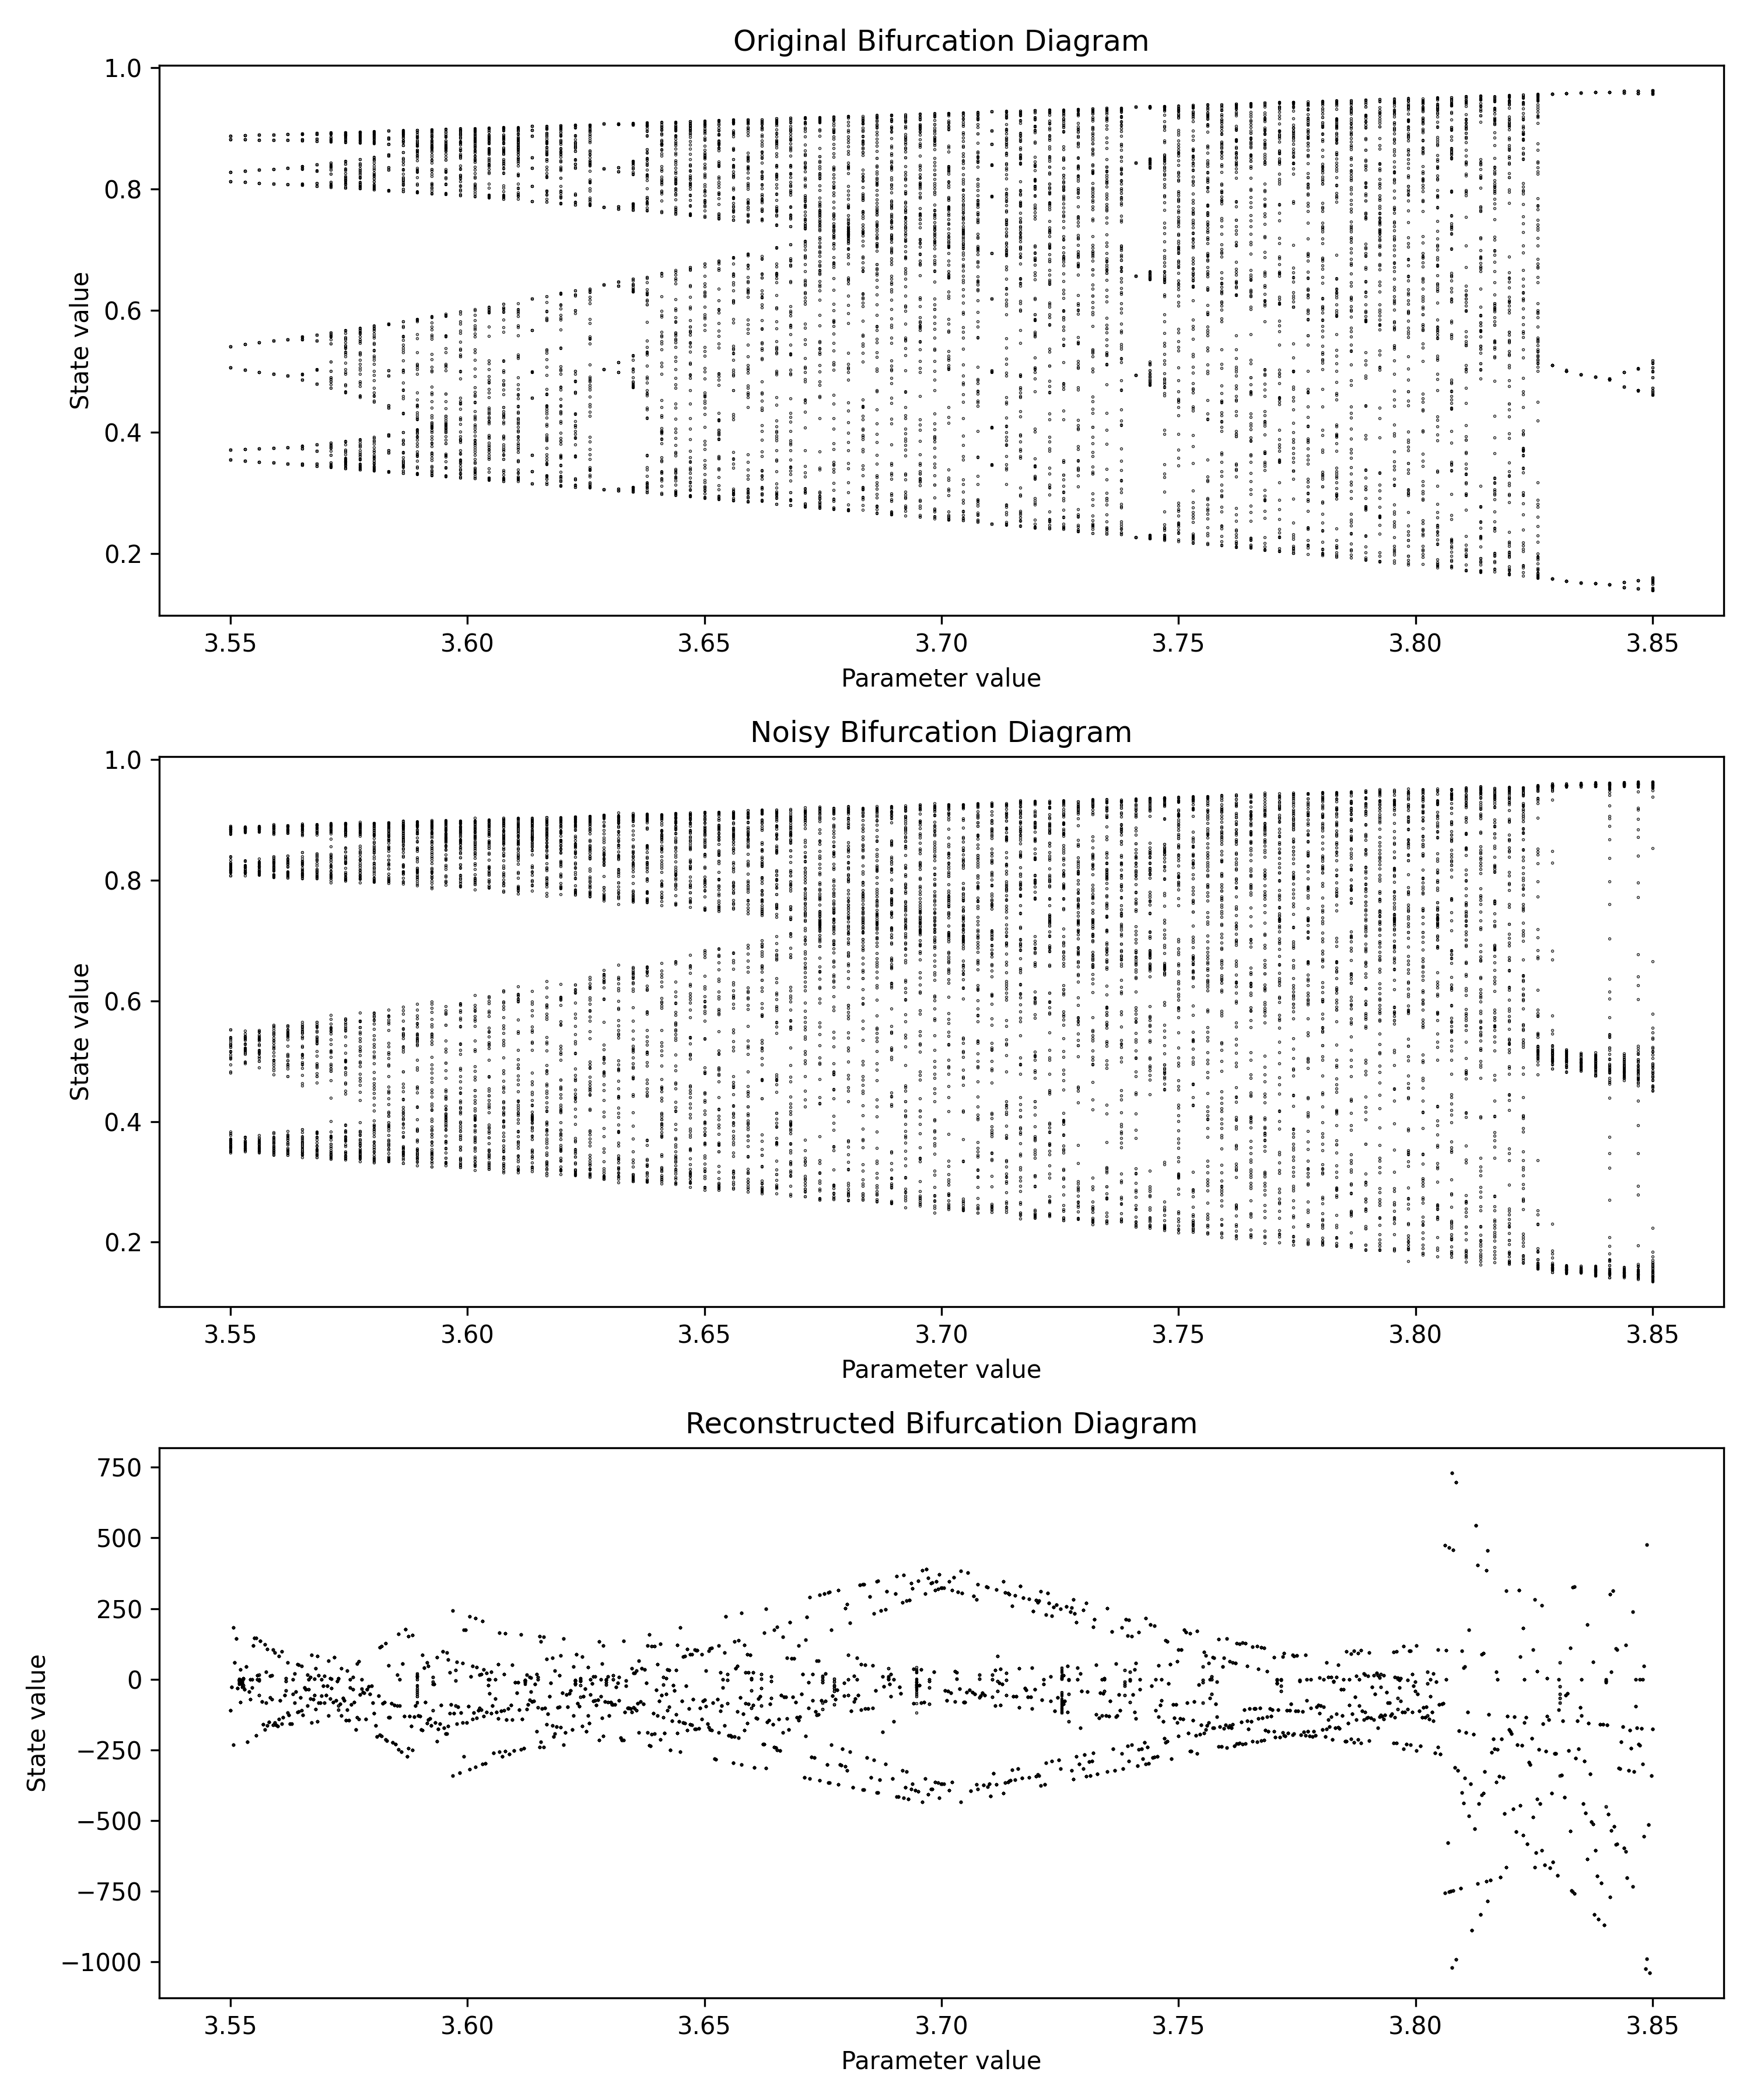
\includegraphics[width=1\linewidth]{figures/bd_reconstruction_elm.png}
\caption{First attempt at reconstruction of bifurcation diagram using reservoir PCA + ELM}
\end{figure}
\end{frame}

\begin{frame}{Bifurcation Reconstruction: Improved Results}
\begin{figure}
\centering
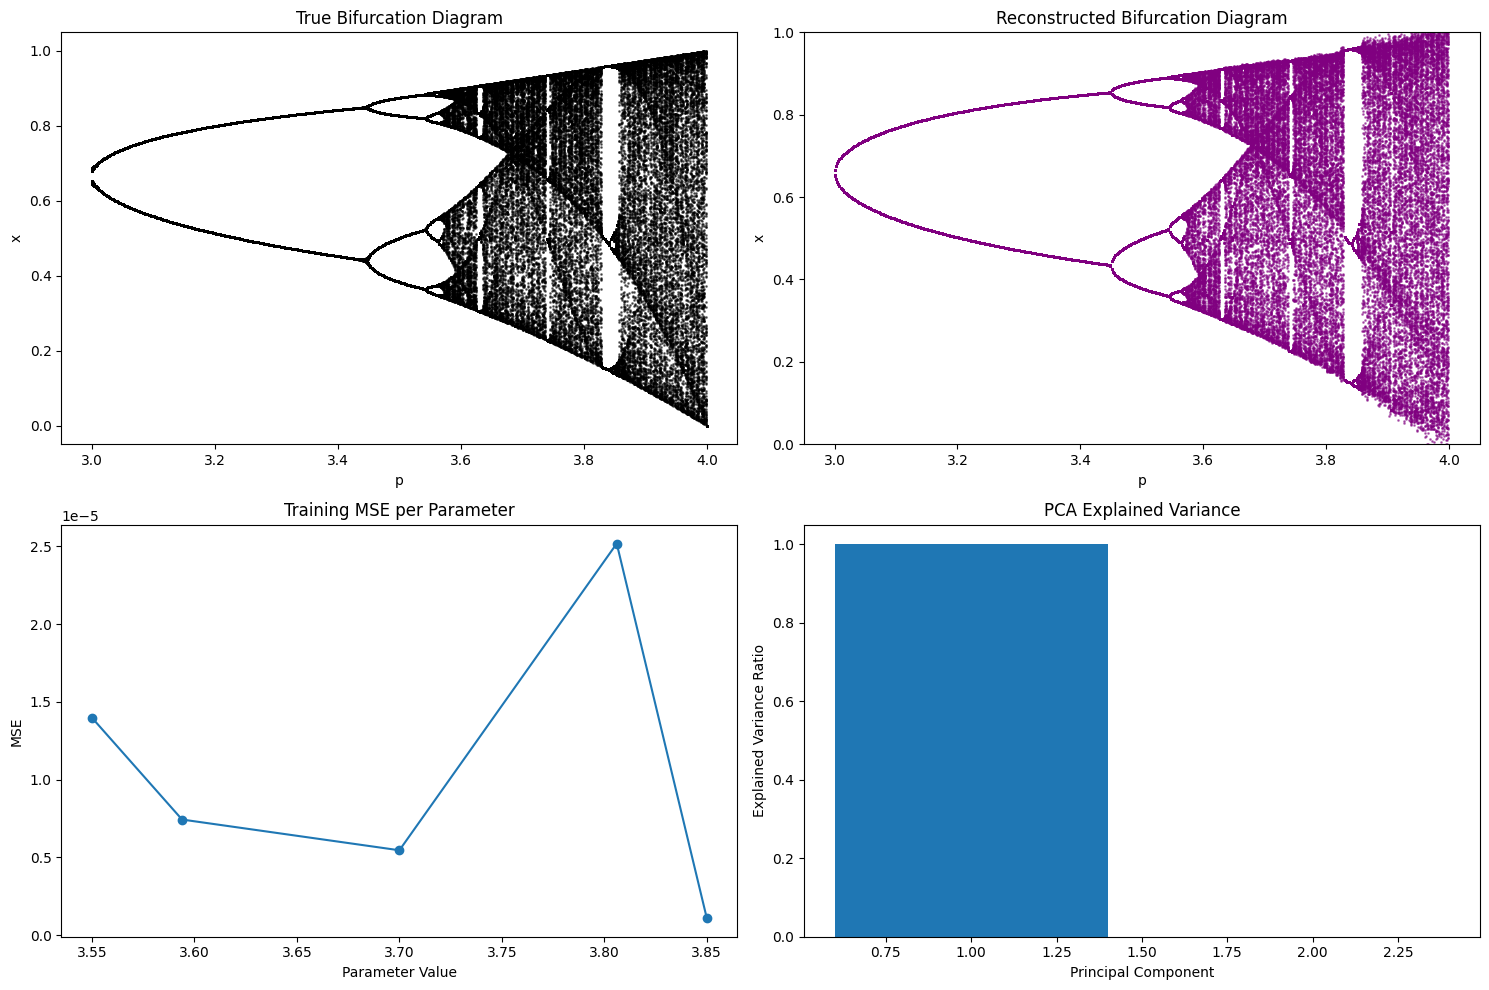
\includegraphics[width=1\linewidth]{figures/bd_1_results.png}
\caption{Improved reconstruction with Training MSE: 1.06e-05}
\end{figure}
\end{frame}

\begin{frame}{Bifurcation Reconstruction: Return Plot}
\begin{figure}
\centering
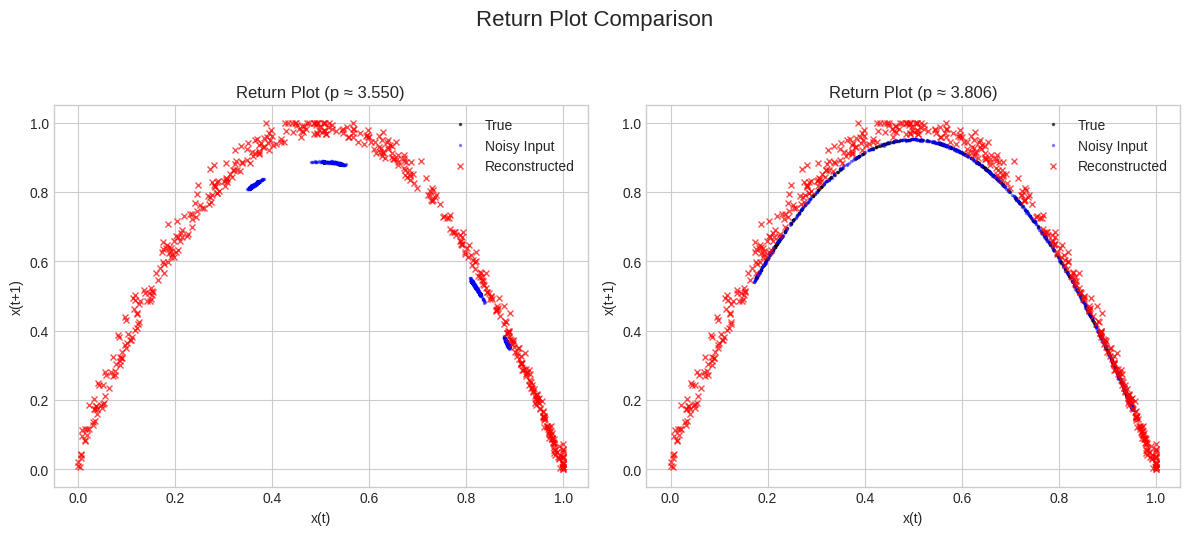
\includegraphics[width=1\linewidth]{figures/bd_return_plot_2.png}
\caption{Reconstructing the return plot, i.e., $x_{(t+1)}$ vs $x_t$}
\end{figure}
\end{frame}

\begin{frame}{Bifurcation Reconstruction: Comparison}
\begin{figure}
\centering
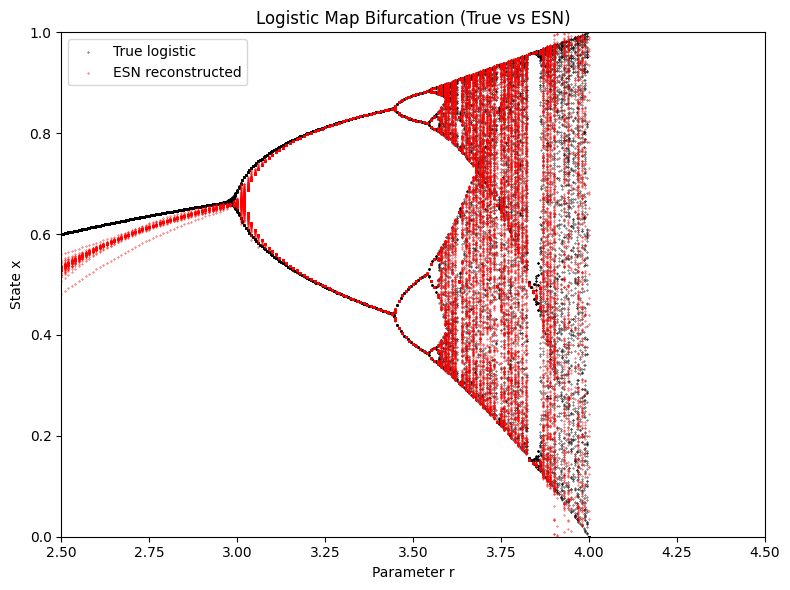
\includegraphics[width=0.8\linewidth]{figures/bf_3_results_overlapped.png}
\caption{Overlapping true and predicted bifurcation diagrams}
\end{figure}
\end{frame}

\begin{frame}{Bifurcation Reconstruction: Lyapunov Exponents}
\begin{figure}
\centering
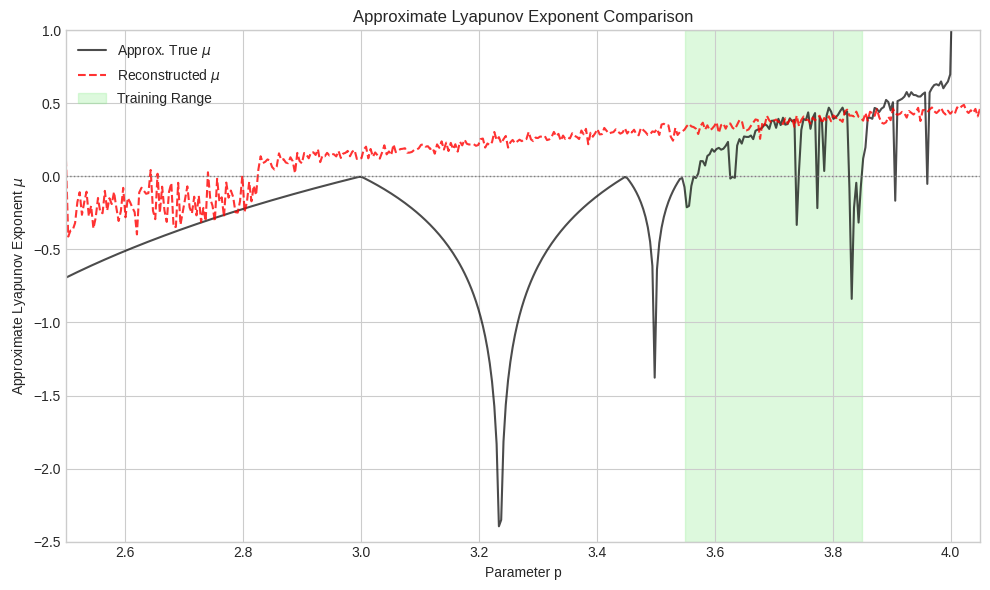
\includegraphics[width=1\linewidth]{figures/lyapanov_bd_rd.png}
\caption{Estimating Lyapunov exponents for different parameter values}
\end{figure}
\end{frame}

\begin{frame}{PCA Component Analysis}
\begin{figure}
\centering
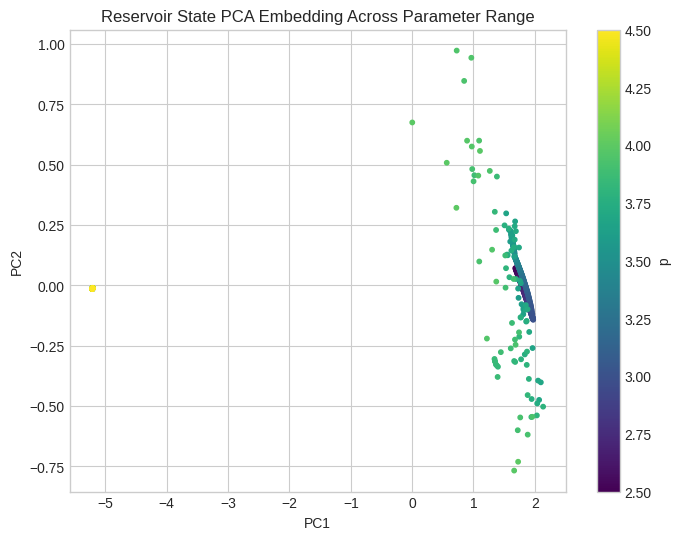
\includegraphics[width=0.8\linewidth]{figures/bd_elm_pca_analysis.png}
\caption{Analysis of PCA components for different parameters}
\end{figure}
\end{frame}

\begin{frame}{Recurrent Networks for Reconstruction}
\begin{itemize}
\item LSTM network as alternative approach
\item Key differences enabling better performance:
    \begin{itemize}
    \item Parameter as explicit input
    \item Learning conditional dynamics
    \item End-to-end training
    \item Reconstruction via iteration
    \end{itemize}
\end{itemize}
\begin{figure}
\centering
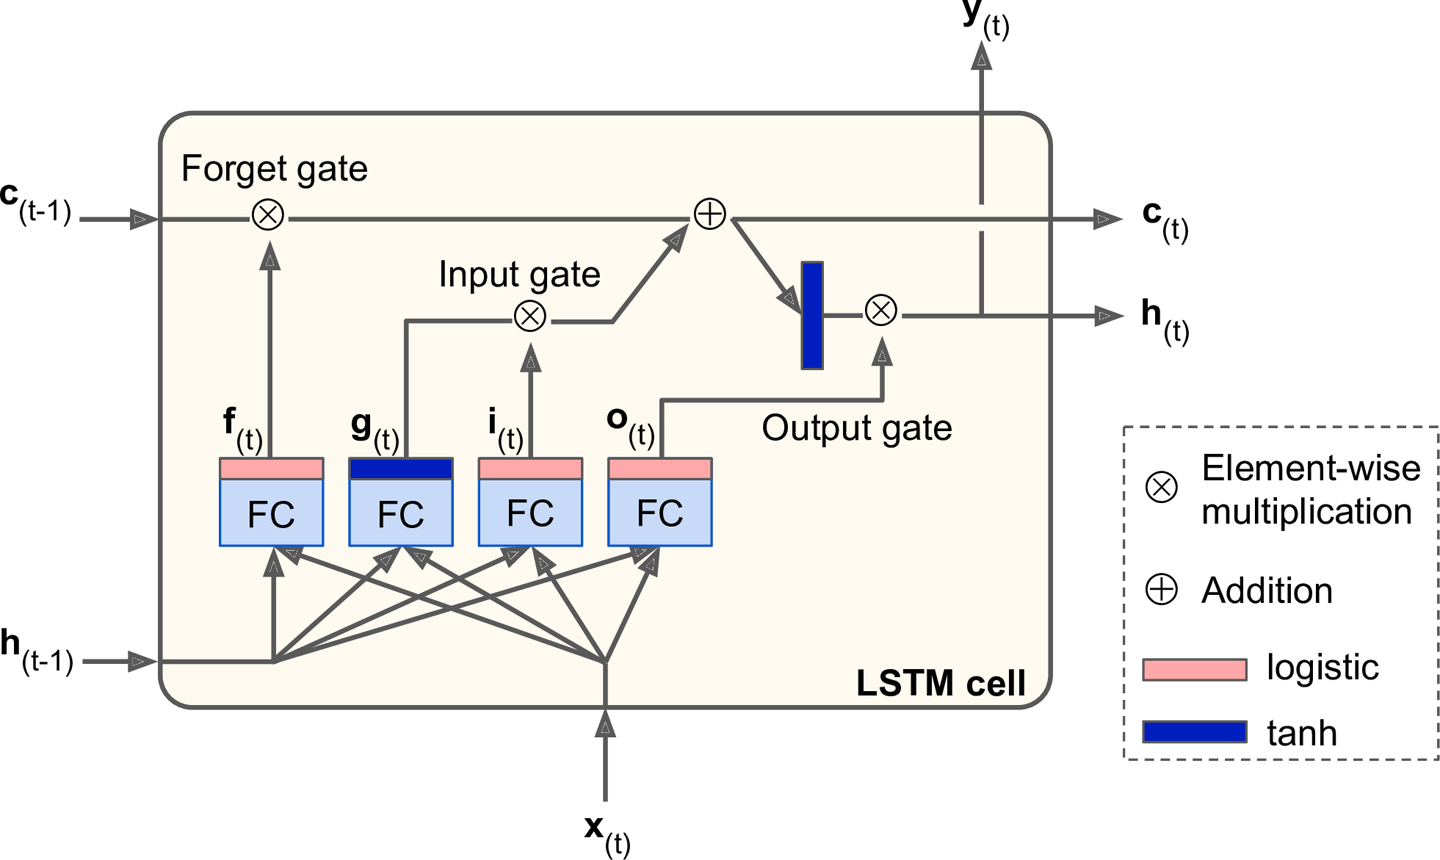
\includegraphics[width=0.8\linewidth]{figures/LSTM_arch.png}
\caption{Long Short-Term Memory (LSTM) architecture}
\end{figure}
\end{frame}

\begin{frame}{LSTM: Bifurcation Diagram Reconstruction}
\begin{figure}
\centering
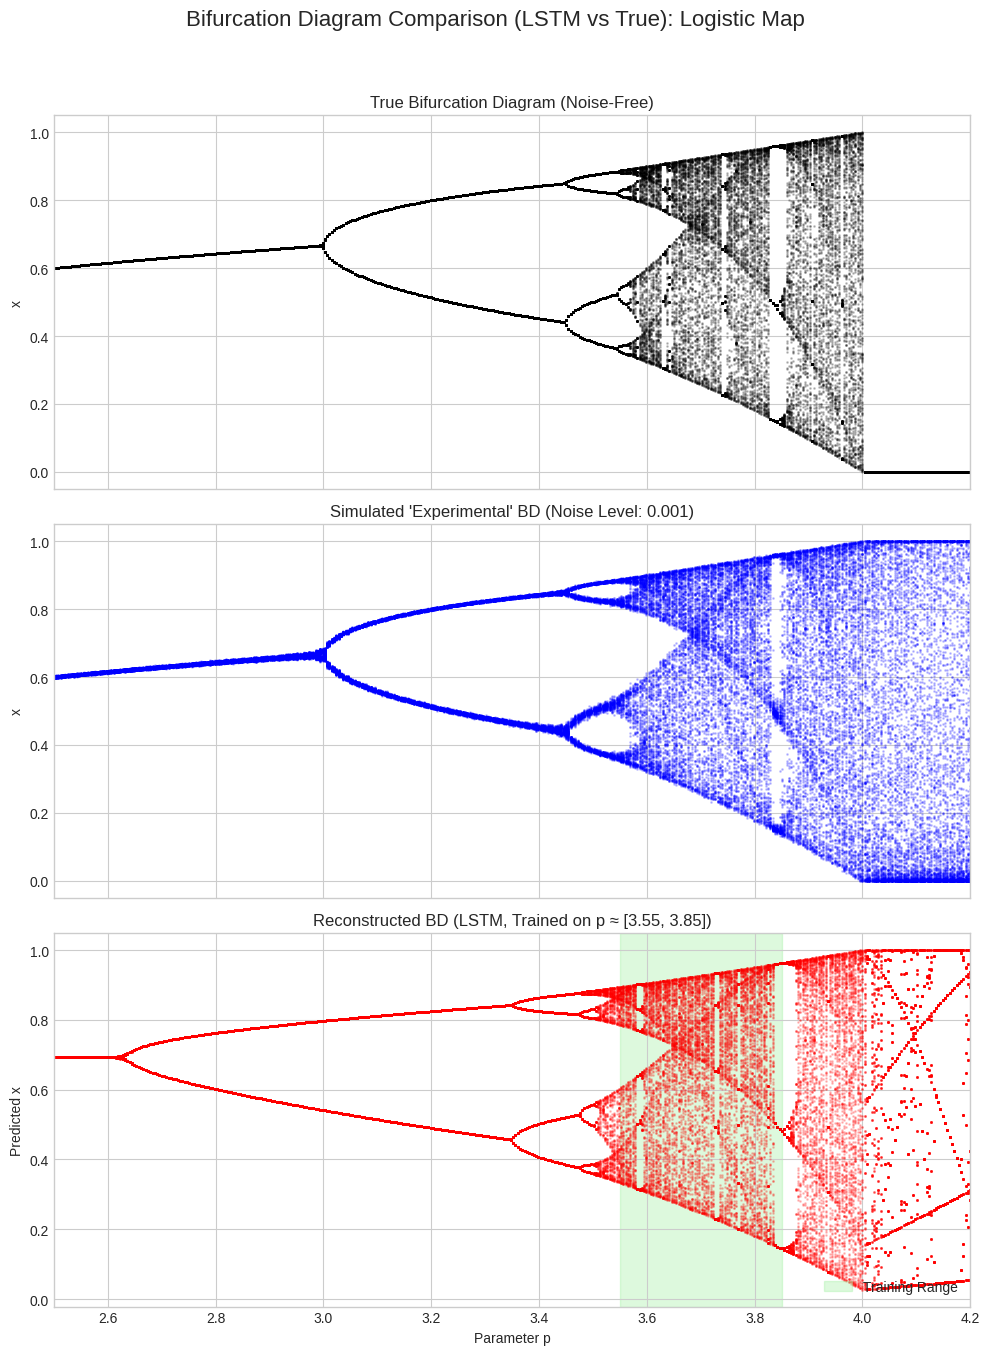
\includegraphics[width=1.0\linewidth]{figures/lstm_bd_1.png}
\caption{Reconstruction using LSTM (green region = training data)}
\end{figure}
\end{frame}

\begin{frame}{LSTM: Return Plot Reconstruction}
\begin{figure}
\centering
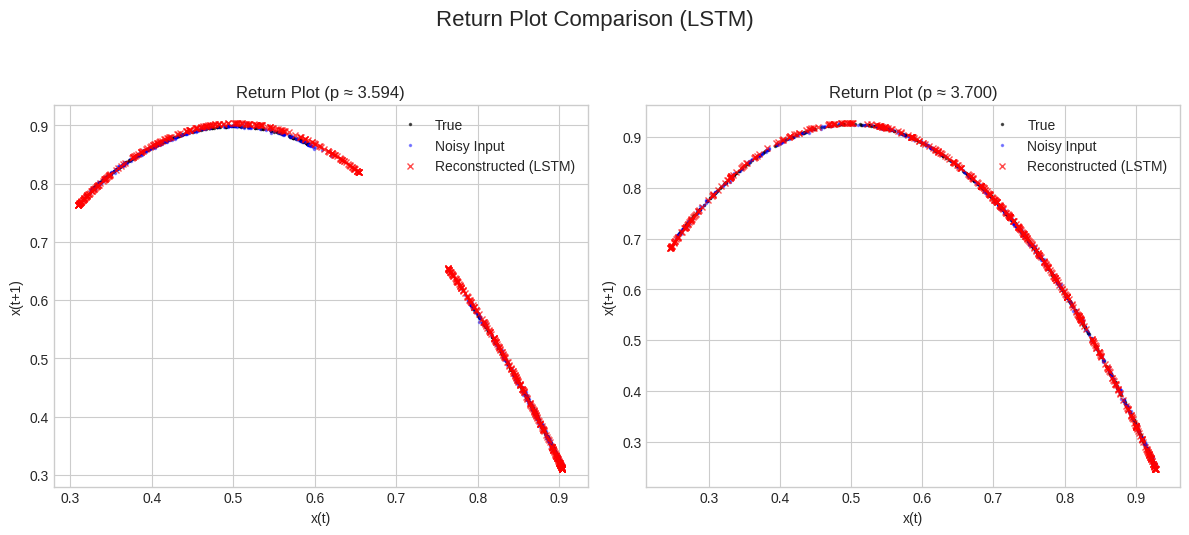
\includegraphics[width=1\linewidth]{figures/lstm_bd_2.png}
\caption{Reconstruction of evolution of $x_{(t+1)}$ vs $x_t$ for different parameter values}
\end{figure}
\end{frame}

\begin{frame}{LSTM vs. ELM Performance}
\begin{itemize}
\item LSTM model: ≈ \textbf{46 seconds} to train
\item Regression ELM: \textbf{less than a second}
\item Performance difference highlights RC's computational efficiency
\item But modern compute resources make sequential models increasingly viable:
    \begin{itemize}
    \item RNNs
    \item Transformers
    \item State Space Models (Mamba)
    \end{itemize}
\end{itemize}
\end{frame}

% Conclusion section
\section{Conclusion}

\begin{frame}{Conclusion}
\begin{itemize}
\item Successfully explored reservoir computing applications:
    \begin{itemize}
    \item ELM + PCA for bifurcation diagram reconstruction
    \item Tested on logistic map as case study
    \end{itemize}
\item Reproduced broad features of period-doubling route to chaos
\item Limitations identified:
    \begin{itemize}
    \item Failed to capture fine structures in chaotic regions
    \item Limited extrapolation beyond training parameter range
    \item Sensitivity to hyperparameter configurations
    \end{itemize}
\end{itemize}
\end{frame}

\begin{frame}{Insights Gained}
\begin{itemize}
\item Learned core RC principles:
    \begin{itemize}
    \item Training efficiency compared to traditional networks
    \item Ability to model nonlinear systems from time-series data
    \end{itemize}
\item Identified advantageous scenarios:
    \begin{itemize}
    \item Processing temporal information with minimal training
    \item Working with physical systems where clean data or precise models are difficult
    \end{itemize}
\item Trade-offs evident:
    \begin{itemize}
    \item Simpler training vs. extrapolation capability
    \item Need for tuning and potentially hybrid methods
    \end{itemize}
\end{itemize}
\end{frame}

% Future Work section
\section{Future Work}

\begin{frame}{Future Work}
\begin{itemize}
\item Improve fidelity and robustness:
    \begin{itemize}
    \item Optimize RC hyperparameters
    \item Apply Bayesian optimization techniques
    \end{itemize}
\item Expand to wider array of dynamical systems:
    \begin{itemize}
    \item Higher-dimensional maps
    \item Continuous-time systems
    \item Different bifurcation types
    \item Coupled systems
    \end{itemize}
\item Compare with alternative RC architectures:
    \begin{itemize}
    \item Deep reservoir networks
    \item Different readout mechanisms
    \end{itemize}
\item Validate with physical hardware data
\end{itemize}
\end{frame}

\begin{frame}{Acknowledgements}
\begin{center}
\Large Thank you for your attention!
\vspace{1cm}

\normalsize
Special thanks to \textbf{Prof. Gaurav Dar} for guidance, insights, and motivation throughout this project.
\end{center}
\end{frame}

\end{document}
